%%%%%%%%%%%%%%%%%%%%%%%%%%%%%%%%%%%%%%%%%
% Short Sectioned Assignment
% LaTeX Template
% Version 1.0 (5/5/12)
%
% This template has been downloaded from:
% http://www.LaTeXTemplates.com
%
% Original author:
% Frits Wenneker (http://www.howtotex.com)
%
% License:
% CC BY-NC-SA 3.0 (http://creativecommons.org/licenses/by-nc-sa/3.0/)
%
%%%%%%%%%%%%%%%%%%%%%%%%%%%%%%%%%%%%%%%%%

%--------------------------------------------------------------------------------
%	PACKAGES AND OTHER DOCUMENT CONFIGURATIONS
%--------------------------------------------------------------------------------

\documentclass[paper=a4, fontsize=11pt]{scrartcl} % A4 paper and 11pt font size

\usepackage{graphicx, float}
\usepackage{caption}
\usepackage{subcaption}
\usepackage[T1]{fontenc} % Use 8-bit encoding that has 256 glyphs
\usepackage{fourier} % Use the Adobe Utopia font for the document - comment this line to return to the LaTeX default
\usepackage[english]{babel} % English language/hyphenation
\usepackage{amsmath,amsfonts,amsthm} % Math packages

\usepackage{sectsty} % Allows customizing section commands
\allsectionsfont{\centering \normalfont\scshape} % Make all sections centered, the default font and small caps

\usepackage{fancyhdr} % Custom headers and footers
\pagestyle{fancyplain} % Makes all pages in the document conform to the custom headers and footers
\fancyhead{} % No page header - if you want one, create it in the same way as the footers below
\fancyfoot[L]{} % Empty left footer
\fancyfoot[C]{} % Empty center footer
\fancyfoot[R]{\thepage} % Page numbering for right footer
\renewcommand{\headrulewidth}{0pt} % Remove header underlines
\renewcommand{\footrulewidth}{0pt} % Remove footer underlines
\setlength{\headheight}{13.6pt} % Customize the height of the header

\numberwithin{equation}{section} % Number equations within sections (i.e. 1.1, 1.2, 2.1, 2.2 instead of 1, 2, 3, 4)
\numberwithin{figure}{section} % Number figures within sections (i.e. 1.1, 1.2, 2.1, 2.2 instead of 1, 2, 3, 4)
\numberwithin{table}{section} % Number tables within sections (i.e. 1.1, 1.2, 2.1, 2.2 instead of 1, 2, 3, 4)

\setlength\parindent{0pt} % Removes all indentation from paragraphs - comment this line for an assignment with lots of text

\usepackage[hidelinks]{hyperref}

%----------------------------------------------------------------------------------------
%	TITLE SECTION
%----------------------------------------------------------------------------------------

\newcommand{\horrule}[1]{\rule{\linewidth}{#1}} % Create horizontal rule command with 1 argument of height

\title{
	\normalfont \normalsize
	\textsc{EPFL CS-444 Virtual Reality} \\ [25pt] % Your university, school and/or department name(s)
	\horrule{0.5pt} \\[0.4cm] % Thin top horizontal rule
	\huge File Explorer in Outer Space - FEOS \\ % The assignment title
	\horrule{2pt} \\[0.5cm] % Thick bottom horizontal rule
}

\author{Group 3: Florian Junker, Sidney Bovet} % Your name

\date{\normalsize\today} % Today's date or a custom date

\begin{document}

\maketitle % Print the title


\begin{figure}[H]
	\centering
	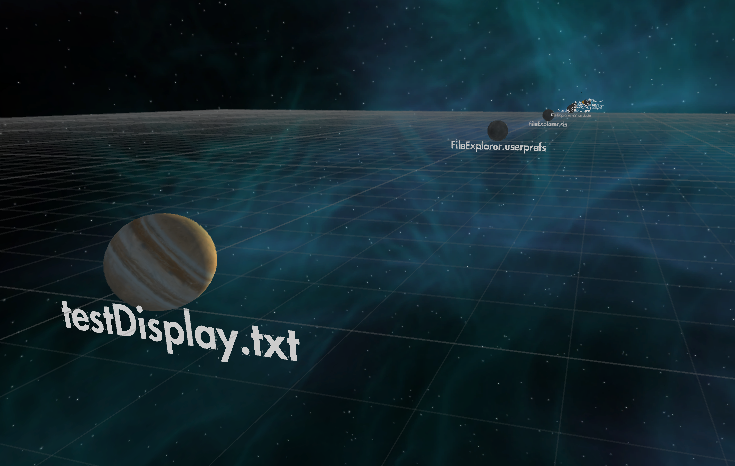
\includegraphics[width=0.8\textwidth]{cover}
\end{figure}

% The report is meant to inform the structure/architecture of your project and instruct on how to configure and run it.


\section{Project presentation \& User experience}


This project aimed to build a 3D file explorer to have an entertaining yet useful VR experience. The base idea is to have all folders represented by solar systems. All files within that folder are planets, whose texture changes according to the file type itself. Figure \ref{fig:general} show a general example of the left eye of the user's view.

\begin{figure}[H]
	\centering
	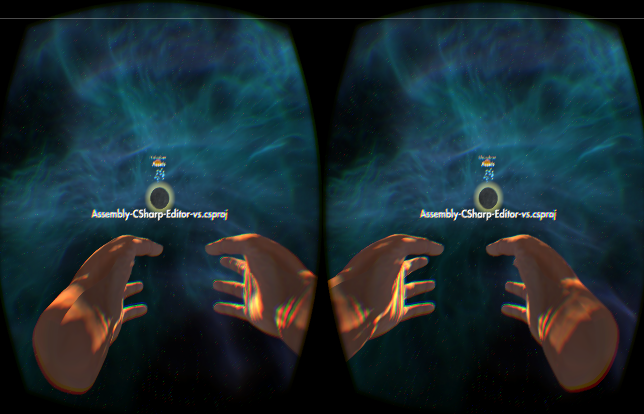
\includegraphics[width=0.5\textwidth]{base-idea}
	\caption{A general screenshot of the file explorer's scenario and GUI.}
	\label{fig:general}
\end{figure}

Immersion in the VE is provided by two devices: a HMD and a Razer Hydra. The former provides a 360-degree field of regard as opposed to other webcam-based head tracking solutions, while the latter gives 6 DOF, occlusion-resistant hand tracking. By coupling the Razor hydra with virtual hands animated according to some trigger buttons pressed, one can feel quite a good sense of Agency given some training. For instance, the user can grab the air using both bottommost triggers to pull and push herself along the axis on which the planets appear. An asteroid belt is used to show the user that the end of the folder has been reached.

\begin{figure}[H]
	\centering
	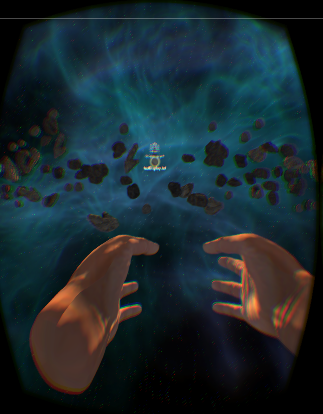
\includegraphics[width=0.5\textwidth]{asteroids}
	\caption{The asteroid belt at the end of the folder.}
	\label{fig:asteroids}
\end{figure}

Selection is achieved through regard: the last item that have crossed the centre of the screen if selected (i.e. simple click on a regular file explorer), and one can activate that selection (i.e. double-click) by pressing the topmost trigger and having a swift move towards the desired item.

\begin{figure}[H]
	\centering
	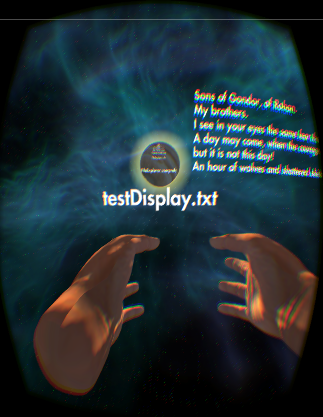
\includegraphics[width=0.5\textwidth]{text-display}
	\caption{How a text file is displayed in the VE.}
	\label{fig:textfile}
\end{figure}

Upon activation (i.e. double-click) a file will either show its content if it is supported (as shown in Figure \ref{fig:textfile} for a text file) or bump to show a negative feedback due to unsupported extension. A folder will trigger a solar system change and the user then can browse that folder.

- How the interaction loop works? What the user sees and how the application behaves with respect to his/her input.

- Relevant screenshot(s) (and/or photos showing the user playing) of the program running

%------------------------------------------------

\section{Libraries, resources and algorithms used}
The virtual environment was built using Unity.

The project uses the Oculus integration plugin for displaying the VE and to achieve head tracking. A modified version of the Hydra framework provided by Razer is used for the tracking of the markers. Full use is made of the various C\# libraries provided by Unity including utilities, math, random, etc.

The physic simulation and particle systems generation mechanisms are those of Unity. For instance the asteroid belt mentioned above is shattered by interacting with the user using Unity's built-in rigid bodies and mesh colliders.

%------------------------------------------------
	
	\section{Understand and compile the project}
	Since the project uses the Sixsense Razor Hydra as a marker tracking system, whose driver is only available for Windows, it is only compatible with a Windows PC. The Oculus and Hydra drivers must be installed on the computer. The version of the different components are the following:
	\begin{description}
		\item[Oculus VR Unity integration] v0.5.0.1-beta
		\item[Sixsense Unity plugin] v1.0.6
		\item[Oculus driver] Windows - v0.5.0.1-beta
		\item[Razer Hydra driver] Windows - v1.01
	\end{description}
	
	
	The whole project can be opened in Unity and compiled from there.
	The unity hierarchy is quiet simple. There is one empty object called controller that contains scripts responsible for planets generation (PlanetController.cs) and SixenseInput.cs that allow us to use razer Hydra controllers. The later is provided by the unity integration and isn't our product. The second game object is the representation of the player that is base on the OVRPlayerController from Oculus Unity integration. UserController a script attached to OVRPlayerController responsible for player movement. We add as child of OVRPlayerController Hands that itself contains RightHand and LeftHand. These three are responsible of everything that is in relation with the razer hydra or the hands animation.\\
	Other game objects are generated by script during the runtime. Typically gameObject that represent files and folders.\\
	The most relevant C\# files to look at in order to understand the project are:
	\begin{description}
		\item[\texttt{planetController.cs}] Located on game object "controller". Generate planets and star clusters according to a given filesystem path. It is also responsible for the solar system movement and the file display 
		\item[\texttt{UserController.cs}] Located on game object "OVRPlayerController". Controls player movements.
		\item[\texttt{SixenseHand}] Located on game object "OVRPlayerController/Hands/RightHand(LeftHand)". Animate the hand and detects controller movement corresponding to action.
		\item[\texttt{SicenseHandsController}] Located on game object "OVRPlayerController/Hands". Handle some over movement that need both hands and correspond to action.
	\end{description}
	
	Once compiled, the \texttt{FileExplorerDirectToRift.exe} file can then be launched to run the file explorer.
	
	Maybe include a diagram and code snippets?
	
	%------------------------------------------------

\section{Discussion \& Conclusion}

During this project we learned a lot of thing regarding the field of VR itself and more generally concerning this kind of creative projects. Given the time this project was supposed to take we had to leave aside lots of improvements we discussed along the path, such as being able to launch executable applications, display images and videos, and so on. On the other hand we believe our code is ready to house these features since we made it in a clear and modulated fashion.

What was good about this project was not to have to stumble upon OpenGL issues and really being able to focus on the VR side of the project. On the other hand it was unclear how much time, effort and quality was expected, which has led us to quite a large workload.

%----------------------------------------------------------------------------------------

\end{document}
